\pagestyle{pippo}
\chapter{HDF dataset and database reader creation}

In a tool for preliminary design phase of an aircraft, it's very important to have aviable database. It's possible to create database starting from graphics using external software. In this appendix will be explained the step required in order to digitalize the graphics, create an HDF dataset and set up the database-reader class in Jpad.

\section{Chart Digitization}
The first step required for create a dataset is to digitalize a chart. Often data is found presented in reports and references as functional X-Y type scatter or line plots. In order to use this data, it must somehow be digitized. This is made with an external software, such as {\itshape Plot Digitizer}. Plot Digitizer is a Java program used to digitize scanned plots of functional data. This program will allow you to take a scanned image of a plot (in GIF, JPEG, or PNG format) and quickly digitize values off the plot just by clicking the mouse on each data point.\cite{plotdigitizer}

\begin{figure}[H]
\centering
{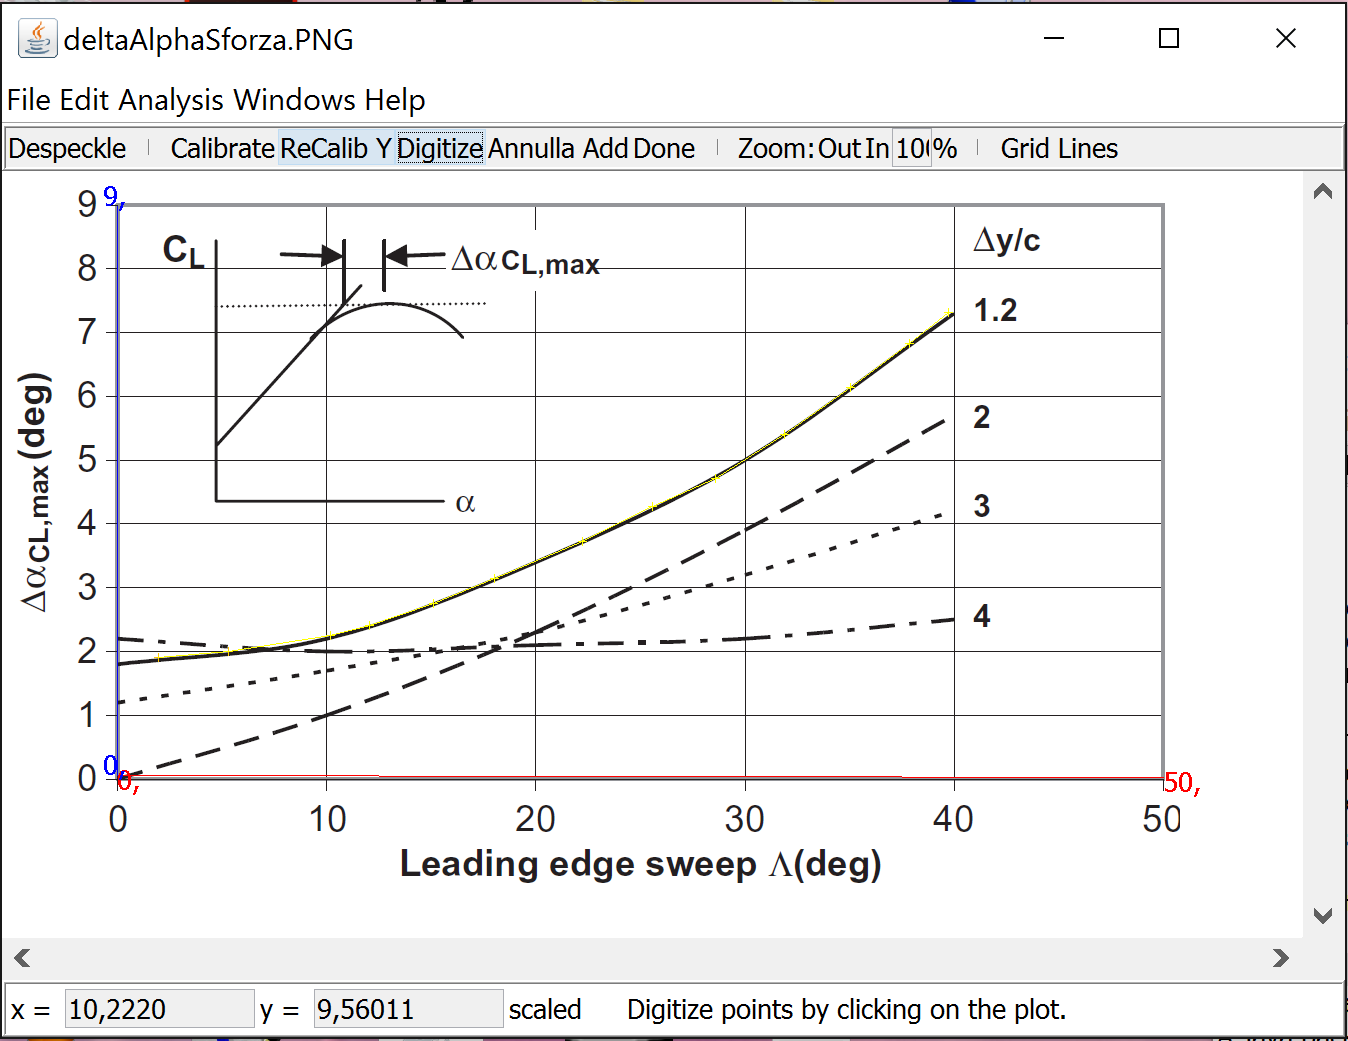
\includegraphics[height=7.9cm]{Immagini/digitize.png}} 
\caption{Chart digitization using Plot Digitizer.}
\label{angles}
\end{figure} 


In order to digitize a chart, first of all it's necessary to calibrate the axis. Plot Digitizer works with both linear and logarithmic axis scales. After it's possible to digitize a curve simply click o it. The values obtained can then be saved to a tex file or .csv file.


\section{Creation of an HDF file with Matlab}

Obtained the .csv file from digitization is necessary to create the HDF file. First of all it's necessary to import the file with couple of coordinates as matrix. After saving the imported files as .mat file, Matlab code comes in play to manage these data and to generate the digitalized curves and the HDF dataset.  The code interpolates curves points with cubic splines in order to have more points to plot for each curve.

\bigskip
\lstset{language=Matlab}
\begin{lstlisting}[frame=rbl,caption={{\footnotesize MATLAB script for creating the HDF Database}},label= [style=\bfseries]{Listing}]
clc; close all; clear all;

%% Import data
DeltaAlphaCLmax_vs_LambdaLE_dy1p2 = importdata('DeltaAlphaCLmax_vs_LambdaLE_dy1p2.mat');
DeltaAlphaCLmax_vs_LambdaLE_dy2p0 = importdata('DeltaAlphaCLmax_vs_LambdaLE_dy2p0.mat');
DeltaAlphaCLmax_vs_LambdaLE_dy3p0 = importdata('DeltaAlphaCLmax_vs_LambdaLE_dy3p0.mat');
DeltaAlphaCLmax_vs_LambdaLE_dy4p0 = importdata('DeltaAlphaCLmax_vs_LambdaLE_dy4p0.mat');

nPoints = 30;
lambdaLEVector_deg = transpose(linspace(0, 40, nPoints));

%% dy/c = 1.2
smoothingParameter = 0.999999;
DAlphaVsLambdaLESplineStatic_Dy1p2 = csaps( ...
    DeltaAlphaCLmax_vs_LambdaLE_dy1p2(:,1), ...
    DeltaAlphaCLmax_vs_LambdaLE_dy1p2(:,2), ...
    smoothingParameter ...
    );

DAlphaVsLambdaLEStatic_Dy1p2 = ppval( ...
    DAlphaVsLambdaLESplineStatic_Dy1p2, ...
    lambdaLEVector_deg ...
    );

%% dy/c = 2.0

smoothingParameter = 0.999999; 
DAlphaVsLambdaLESplineStatic_Dy2p0 = csaps( ...
    DeltaAlphaCLmax_vs_LambdaLE_dy2p0(:,1), ...
    DeltaAlphaCLmax_vs_LambdaLE_dy2p0(:,2), ...
    smoothingParameter ...
    );

DAlphaVsLambdaLEStatic_Dy2p0 = ppval( ...
    DAlphaVsLambdaLESplineStatic_Dy2p0, ...
    lambdaLEVector_deg ...
    );

%% dy/c = 3.0

smoothingParameter =0.999999;
DAlphaVsLambdaLESplineStatic_Dy3p0 = csaps( ...
    DeltaAlphaCLmax_vs_LambdaLE_dy3p0(:,1), ...
    DeltaAlphaCLmax_vs_LambdaLE_dy3p0(:,2), ...
    smoothingParameter ...
    );

DAlphaVsLambdaLEStatic_Dy3p0 = ppval( ...
    DAlphaVsLambdaLESplineStatic_Dy3p0, ...
    lambdaLEVector_deg ...
    );

%% dy/c = 4.0

smoothingParameter = 0.999999; 
DAlphaVsLambdaLESplineStatic_Dy4p0 = csaps( ...
    DeltaAlphaCLmax_vs_LambdaLE_dy4p0(:,1), ...
    DeltaAlphaCLmax_vs_LambdaLE_dy4p0(:,2), ...
    smoothingParameter ...
    );

DAlphaVsLambdaLEStatic_Dy4p0 = ppval( ...
    DAlphaVsLambdaLESplineStatic_Dy4p0, ...
    lambdaLEVector_deg ...
    );


%% Plots
figure(1)
plot ( ...
    lambdaLEVector_deg, DAlphaVsLambdaLEStatic_Dy1p2, '-*b' ... , ...
 );
 hold on
 
 plot ( ...
    lambdaLEVector_deg, DAlphaVsLambdaLEStatic_Dy2p0, '-b' ... , ...
 );

hold on

plot ( ...
    lambdaLEVector_deg, DAlphaVsLambdaLEStatic_Dy3p0, '*b' ... , ...
 );

hold on

plot ( ...
    lambdaLEVector_deg, DAlphaVsLambdaLEStatic_Dy4p0, 'b' ... , ...
 );

 xlabel('\Lambda_{le} (deg)'); ylabel('\Delta\alpha_{C_{L,max}}');
 title('Angle of attack increment for wing maximum lift in subsonic flight');
  legend('\Delta y/c = 1.2', '\Delta y/c = 2.0', '\Delta y/c = 3.0','\Delta y/c = 4.0');
 axis([0 50 0 9]);
 grid on;
 

 
%% preparing output to HDF

% dy/c
dyVector = [ ...
    1.2;2.0;3.0;4.0 ...
    ];

%columns --> curves
myData = [ ...
    DAlphaVsLambdaLEStatic_Dy1p2,...
        DAlphaVsLambdaLEStatic_Dy2p0, ... % -> 2
        DAlphaVsLambdaLEStatic_Dy3p0, ... % -> 3
        DAlphaVsLambdaLEStatic_Dy4p0];    % -> 4

hdfFileName = 'DAlphaVsLambdaLEVsDy.h5';

if ( exist(hdfFileName, 'file') )
    fprintf('file %s exists, deleting and creating a new one\n', hdfFileName);
    delete(hdfFileName)
else
    fprintf('Creating new file %s\n', hdfFileName);
end

% Dataset: data
h5create(hdfFileName, '/DAlphaVsLambdaLEVsDy/data', size(myData'));
h5write(hdfFileName, '/DAlphaVsLambdaLEVsDy/data', myData');

% Dataset: var_0
h5create(hdfFileName, '/DAlphaVsLambdaLEVsDy/var_0', size(dyVector'));
h5write(hdfFileName, '/DAlphaVsLambdaLEVsDy/var_0', dyVector');

% Dataset: var_1
h5create(hdfFileName, '/DAlphaVsLambdaLEVsDy/var_1', size(lambdaLEVector_deg'));
h5write(hdfFileName, '/DAlphaVsLambdaLEVsDy/var_1', lambdaLEVector_deg');
\end{lstlisting}

\noindent \\ \\ 
This script plot the graph after digitization. In this way it's possible to compare the initial graph and the digitized one.

\pagestyle{pippo}
 \begin{figure}[H]
\centering
{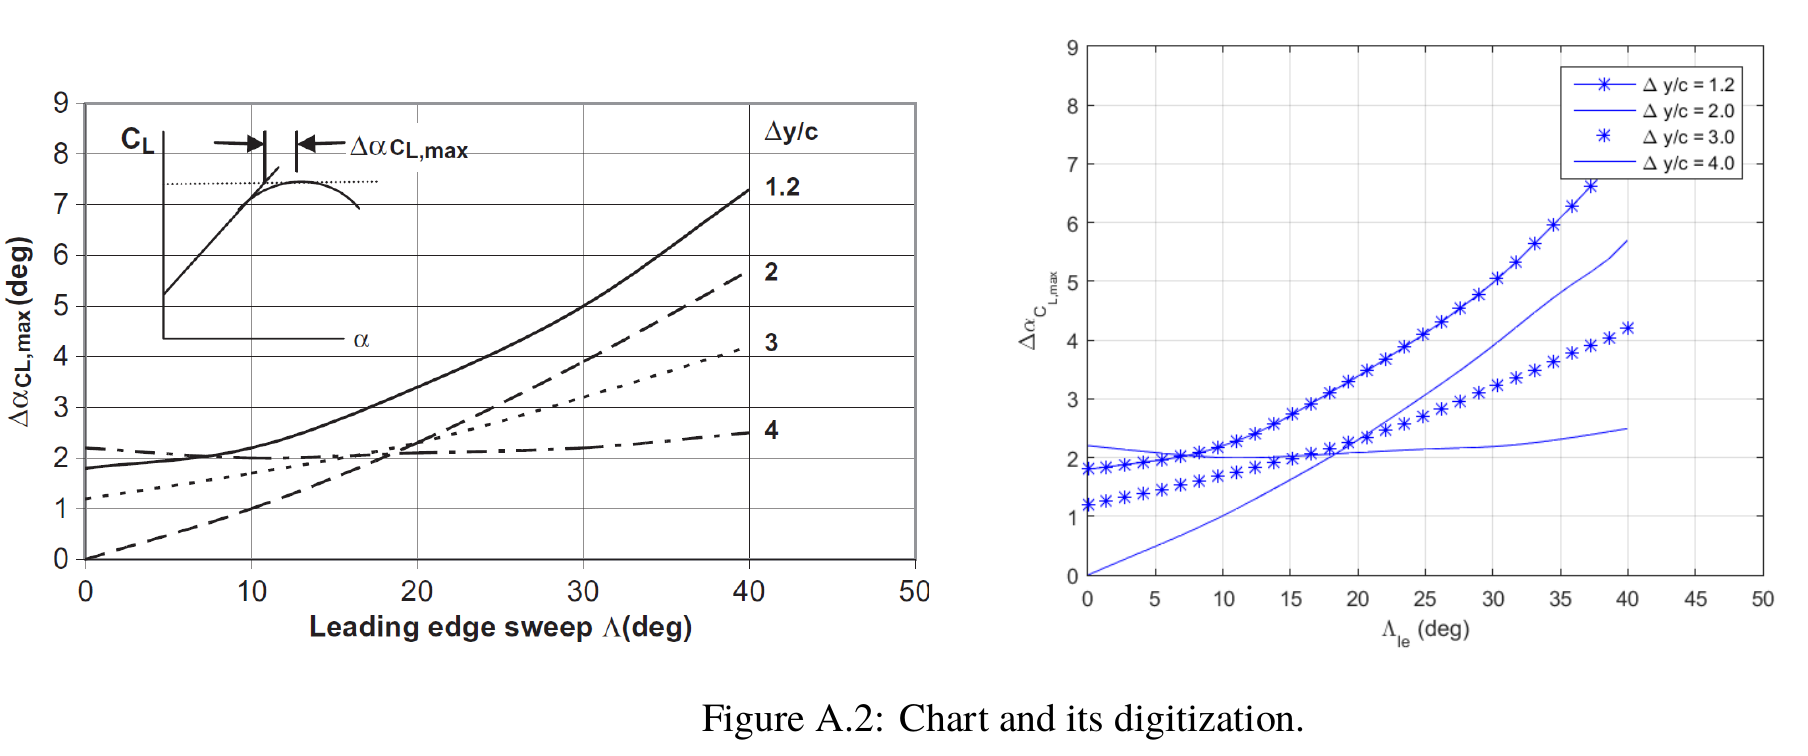
\includegraphics[height=6cm]{Immagini/digitize2.png}} 
\label{angles}
\end{figure} 

\chapter{App2}



